\chapter{An Efficient, Scalable and Exact Representation of High-Dimensional Color Information Enabled via de Bruijn Graph Search}
\label{chap:mantis}


\section{Introduction}\label{sec:intro}

The \longcdbg (\cdbg)~\cite{IqbalCaTu12}, an extension of the classical
\dbg~\citep{pevzner2001eulerian,pevzner2001fragment,chikhi2014representation},
is a key component of a growing number of genomics tools. Augmenting the traditional
\dbg with ``color'' information provides a mechanism to associate meta-data,
such as the raw sample or reference of origin, with each \kmer. Coloring the \dbg
enables it to be used in a wide range of applications, such as large-scale sequence
search~\citep{mantis, Solomon2016Fast, Solomon2017Improved,
Sun2017Allsome, bradley2017real} (though some~\citep{Solomon2016Fast, Solomon2017Improved,Sun2017Allsome}
do not explicitly couch their representations in
the language of the \cdbg), population-level variation
detection~\cite{MuggliBoNo17, holley2016bloom, rainbowfish}, traversal and search
in a pan-genome~\cite{holley2016bloom}, and sequence
alignment~\cite{liu2016debga}. The popularity and applicability of the
\cdbg has spurred research into developing space-efficient and high-performance
data-structure implementations.

An efficient and fast representation of \cdbg requires optimizing both the \dbg and the
color information.  While there exist efficient and scalable methods
for representing the topology of the
\dbg~\cite{chikhi2012space,salikhov2014using,bowe2012succinct,chikhi2014representation,crawford2018practical,PandeyBeJo2017d}
with fast query time, a scalable and exact representation of the color
information has remained a challenge. Recently, ~\citet{doi:10.1093/bioinformatics/bty632}
has tackled this challenge by relaxing the exactness
constraints --- allowing the returned color set for a \kmer to contain extra
samples with some controlled probability --- but it is not immediately clear how
this method can be made exact.

Specifically,  existing exact color representations suffer from large
sizes and a fast growth rate that leads them to dominate the total
representation size of the \cdbg with even a moderate number of input
samples (see~\Cref{fig:asymptotics}).  As a result, the color information grows to
dominate the space used by all these indexes and limits their ability to scale
to large input data sets.

Iqbal et al.\ introduced \cdbgs~\cite{IqbalCaTu12}
and proposed a hash-based representation of the \dbg in which each \kmer is
additionally tagged with the list of reference genomes in which it is contained.

Muggli et al. reduced the size of the \cdbg in VARI~\citep{MuggliBoNo17} by
replacing the hash map with BOSS~\cite{bowe2012succinct} (a BWT-based~\citep{bwt}
encoding of the \dbg that assigns a unique ID to each \kmer) and using a boolean
matrix indexed by the unique \kmer ID and genome reference ID to indicate
occurrence.  They reduced the size of the occurrence matrix by applying
off-the-shelf compression techniques RRR~\cite{RamanRaRa02} and
Elias-Fano~\citep{elias1974efficient} encoding.  Rainbowfish~\cite{rainbowfish}
shrank the color table further by ensuring that rows of the color matrix are
unique, mapping all \kmers with the same color information to a single row, and
assigning row indices based on the frequency of each occurrence pattern.

However, despite these improvements, the scalability of the resulting structure
remains limited because even after eliminating redundant colors, the space for
the color table grows quickly to dominate the total space used by these data
structures.

We observe that, in real biological data, even when the number of distinct color
classes is large, many of them will be near each other in terms of the set of
samples or references they encode. That is, the \ccs tend to be highly
correlated rather than uniformly spread across the space of possible colors.
There are intuitive reasons for such characteristics. For example, we observe
that adjacent \kmers in the \dbg are extremely likely to have either identical
or similar color classes, enabling storage of small deltas instead of the
complete color classes.  This is because \kmers adjacent in the \dbg are likely
to be adjacent (and hence present) in a similar set of input samples. In the
context of sequence-search, because genomes and transcriptomes are largely
preserved across organs, individuals, and even across related species, we expect
two \kmers that occur together in one sample to be highly correlated in their
occurrence across many samples. Thus, we can take advantage of
this correlation when devising an efficient encoding scheme for the \cdbg's
associated color information.


In this paper, we develop a general scheme for efficient and scalable encoding
of the color information in the \cdbg by encoding \ccs (i.e., the patterns of
occurrence of a \kmer in samples) in terms of their differences (which are
small) with respect to some ``neighboring'' \cc.  The key technical
challenge, solved by our work, is efficiently searching for the neighbors of
\ccs in the high-dimensional space of colors by leveraging the observation that
similar color classes tend to be topologically close in the underlying \dbg.  We
construct a weighted graph on the color classes in the \cdbg, where the weight
of each edge corresponds to the space required to store the delta between its
endpoints.  Finding the minimum spanning tree (MST) of this graph gives a
minimal delta-based representation.
Although reconstructing a color class on this representation requires
a walk to the MST root node, abundant temporal locality on the lookups
allows us to use a small cache to mitigate the performance impact,
yielding query throughput that is essentially the same as when all
color classes are represented explicitly.

An alternative would have been to try to limit the depth (or diameter)
of the MST.  This problem is heavily studied in two forms: the
unrooted bounded-diameter MST problem~\cite{Raidl08} and the rooted
hop-constrained MST problem~\cite{AlthausFuHa05}.  Neither is in APX,
i.e., it is not possible to approximate them to within any constant
factor~\cite{ManyemStMa96}.  Althaus et al. gave an $O(\log n)$
approximation assuming the edge weights form a
metric~\cite{AlthausFuHa05}.  Khuller et al. show that, if the edge
\textit{lengths} are the same as the edge \textit{weights}, then there
is an efficient algorithm for finding a spanning tree that is within a
constant of optimal in terms of both diameter and
weight~\cite{KhullerBaNe02}.  Marathe et al. show that in general we
can find trees within $O(\log n)$ of the minimum diameter and
weight~\cite{MaratheRaSu98}.  We can't use Khuller's approach (because our edge
lengths are not equal to our edge weights), and even a $O(\log n)$
approximation would give up a potentially substantial amount of space.


We showcase the generality and applicability of our color class table
compression technique by demonstrating it in two computational biology
applications: sequence search and variation detection.
%
We compare our novel color class table representation with the representation
used in Mantis~\cite{mantis}, a state-of-the-art large-scale sequence-search
tool that uses a \cdbg to index a set of sequencing samples, and the representation used in
Rainbowfish~\citep{rainbowfish}, a state-of-the-art index to
facilitate variation detection over a set of genomes.

We show that our approach maintains the same query
performance while achieving over $11\times$ and $2.5\times$ storage savings
relative to the representation previously used by these tools.

%%%%%%%%%%%%%%%%%%%%%%%%%%%%%%%%%%%%%%%%%%%%%%%%%%%%%%%%%%%%%%%%
%%
%% Methods
%%
%%%%%%%%%%%%%%%%%%%%%%%%%%%%%%%%%%%%%%%%%%%%%%%%%%%%%%%%%%%%%%%%
\section{Methods}
\label{methods}

This section describes our compact \cdbg representation.  We first define \cdbgs
and briefly describe existing compact \cdbg representations.  We then outline
the high-level idea behind our compact representation and explain how we use the
\dbg to efficiently build our compact representation.  Finally, we describe
implementation details and optimizations to our query algorithm.

\subsection{\longCdbgs}
\label{subsec:cdbg}
\dBGs are widely used to represent the topological structure of a set of
\kmers~\cite{pevzner2001eulerian,Simpson09Abyss,SchulzZeVi12,zerbino08velvet,GrabherrHqYa11,ChangLi15,LiuLi16,PandeyBeJo2017d}.
The \dbg induced by a set of \kmers is defined below.

\begin{definition}
    %
    Given a set $E$ of \kmers, the \defn{\dbg induced by $E$} has edge set $E$,
    where each \kmer (or edge) connects its two $(k-1)$-length substrings (or
    vertices).
    %
\end{definition}

\Cdbgs extend the \dbg by assigning a \defn{color class} $C(x)$ to each edge (or
node) $x$ of the \dbg.  The color class $C(x)$ is a set drawn from some universe
$U$.  Examples of $U$ and $C(x)$ are

\begin{itemize}
    \item Sometimes, $U$ is a set of
    reference genomes, and $C(x)$ is the subset of reference genomes
    containing \kmer $x$~\cite{pufferfish,liu2016debga,rainbowfish,MuggliBoNo17}.
    \item Sometimes, $U$ is a set of \defn{reads},
    and $C(x)$ is the subset of reads containing $x$~\citep{mccortex,alipanahi2018resistome,alipanahi2018recoloring}.
    \item Sometimes, $U$ is a set
    of sequencing experiments, and $C(x)$ is the subset of sequencing experiments containing $x$~\cite{mantis, Solomon2016Fast, Solomon2017Improved, Sun2017Allsome}.
\end{itemize}
The goal of a \cdbg representation is to store $E$ and $C$ as
compactly as possible\footnote{The nodes of the \dbg are typical
stored implicitly, because the node set is simply a function of $E$.},
while supporting the following operations efficiently:
\begin{itemize}
    \item \defn{Point query.}  Given a \kmer $x$, determine whether $x$
    is in $E$.
    \item \defn{Color query.} Given a \kmer $x\in E$, return $C(x)$.
\end{itemize}

Given that we can perform point queries, we can traverse the \dbg by
simply querying for the 8 possible predecessor/successor edges of an edge. This enables us
to implement more advanced algorithms, such as bubble calling~\cite{IqbalCaTu12}.

Many \cdbg representations typically decompose, at least logically,
into two structures: one structure storing a \dbg and associating an
ID with each \kmer, and one structure mapping these IDs
to the actual \cc~\cite{MuggliBoNo17,rainbowfish,PandeyBeJo17a}. The individual
color classes can be represented as bit-vectors, lists, or via a hybrid scheme~\citep{seqothello}.
This information is typically compressed~\cite{RamanRaRa02,Ottaviano2014Partitioned,ziv1977universal}.

Our paper follows this standard approach, and focuses exclusively on reducing
the space required for the structure storing the color information. We
propose a compact representation that, given a color ID, can return the
corresponding color efficiently. Although we pair our color table representation
with the \dbg structure representation of the \cqf~\cite{PandeyBeJo17a} as used
in \mantis~\cite{mantis}, our proposed color table
representation can be paired with other \dbg representations.

\subsection{A similarity-based \cdbg representation}

The key observation behind our compressed color-class representation
is that the color classes of \kmers that are adjacent in the \dbg are
likely to be very similar.  Thus, rather than storing each color class
explicitly, we can store only a few color classes explicitly and, for
all the remaining color classes, we store only their differences from
other color classes.  Because the differences are small, the total space
used by the representation will be small.

Motivated by the observation above, we propose to find an encoding of the \ccs
that takes advantage of the fact that most \ccs can be represented in terms of
only a small number of edits (i.e., flipping the parity of only a few bits) with
respect to some neighbor in the high-dimensional space of the \ccs.
%
This idea was first explored by~\citet{Bookstein1991Compression} in the context
of information retrieval. Bookstein and Klein showed how to exploit the implicit
clustering among bitmaps in IR to achieve excellent reduction in storage space to
represent those bitmaps using an MST as the underlying representation.
Unfortunately, the approach taken by Bookstein and Klein cannot be directly used
in our problem, since it requires computing and optimizing upon the full Hamming
distance graph of the bitvectors being represented, which is not tractable for
the scale of data we are analyzing.  Hence, what we need is a method to efficiently
discover an incomplete and highly-sparse Hamming distance graph that, nonetheless,
supports a low-weight spanning tree.
%
We describe below how we apply and modify this approach in the context of the
set of correlated bit vectors (i.e., \ccs) that we wish to encode.

We construct our compressed color class representation as follows
(see \Cref{fig:mstConstruction}).
For each edge $x$ of the \dbg, let $C(x)$ be the color class of $x$.
Let $\calC$ be the set of all \ccs that occur in the \dbg.  We first
construct an undirected graph with vertex set $\calC$ and edge set reflecting the
adjacency relationship implied by the \dbg.  In other words, there is
an edge between color classes $c_1$ and $c_2$ if there exist adjacent
edges (i.e., incident on the same node) $x$ and $y$ in the \dbg such
that $c_1=C(x)$ and $c_2=C(y)$.  These edges indicate color classes
that are likely to be similar, based on the structure of the \dbg.  We
then add a special node $\emptyset$ to the color class graph, which is
connected to every node.  We set the weight of every edge in the color
class graph to be the Hamming distance between its two endpoints
(where we view color classes as bit vectors and $\emptyset$ is the
all-zeros bit vector).

We then compute a minimum spanning tree of the color class graph and
root the tree at the special $\emptyset$ node.  Note that, because the $\emptyset$
node is connected to every other node in the graph, the graph is
connected and hence an MST is guaranteed to exist.  By using a minimum
spanning tree, we minimize the total size of the differences that
we need to store in our compressed representation.

We then store the MST as a table mapping each color class ID to the ID
of its parent in the MST, along with a list of the differences between
the color class and its parent.  For convenience we can view the list
of differences between color class $c_1$ and color class $c_2$ as a
bit vector $c_1 \oplus c_2$, where $\oplus$ is the bit-wise
exclusive-or operation.  To reconstruct a color class given its ID $i$,
we simply xor all the difference vectors we encounter while walking
from $i$ to the root of the MST.

\begin{figure*}[t!]
    \captionsetup[subfigure]{justification=justified}
    \centering
    \begin{subfigure}[t]{0.49\textwidth}
        \captionsetup{width=0.7\columnwidth}
        \centering
        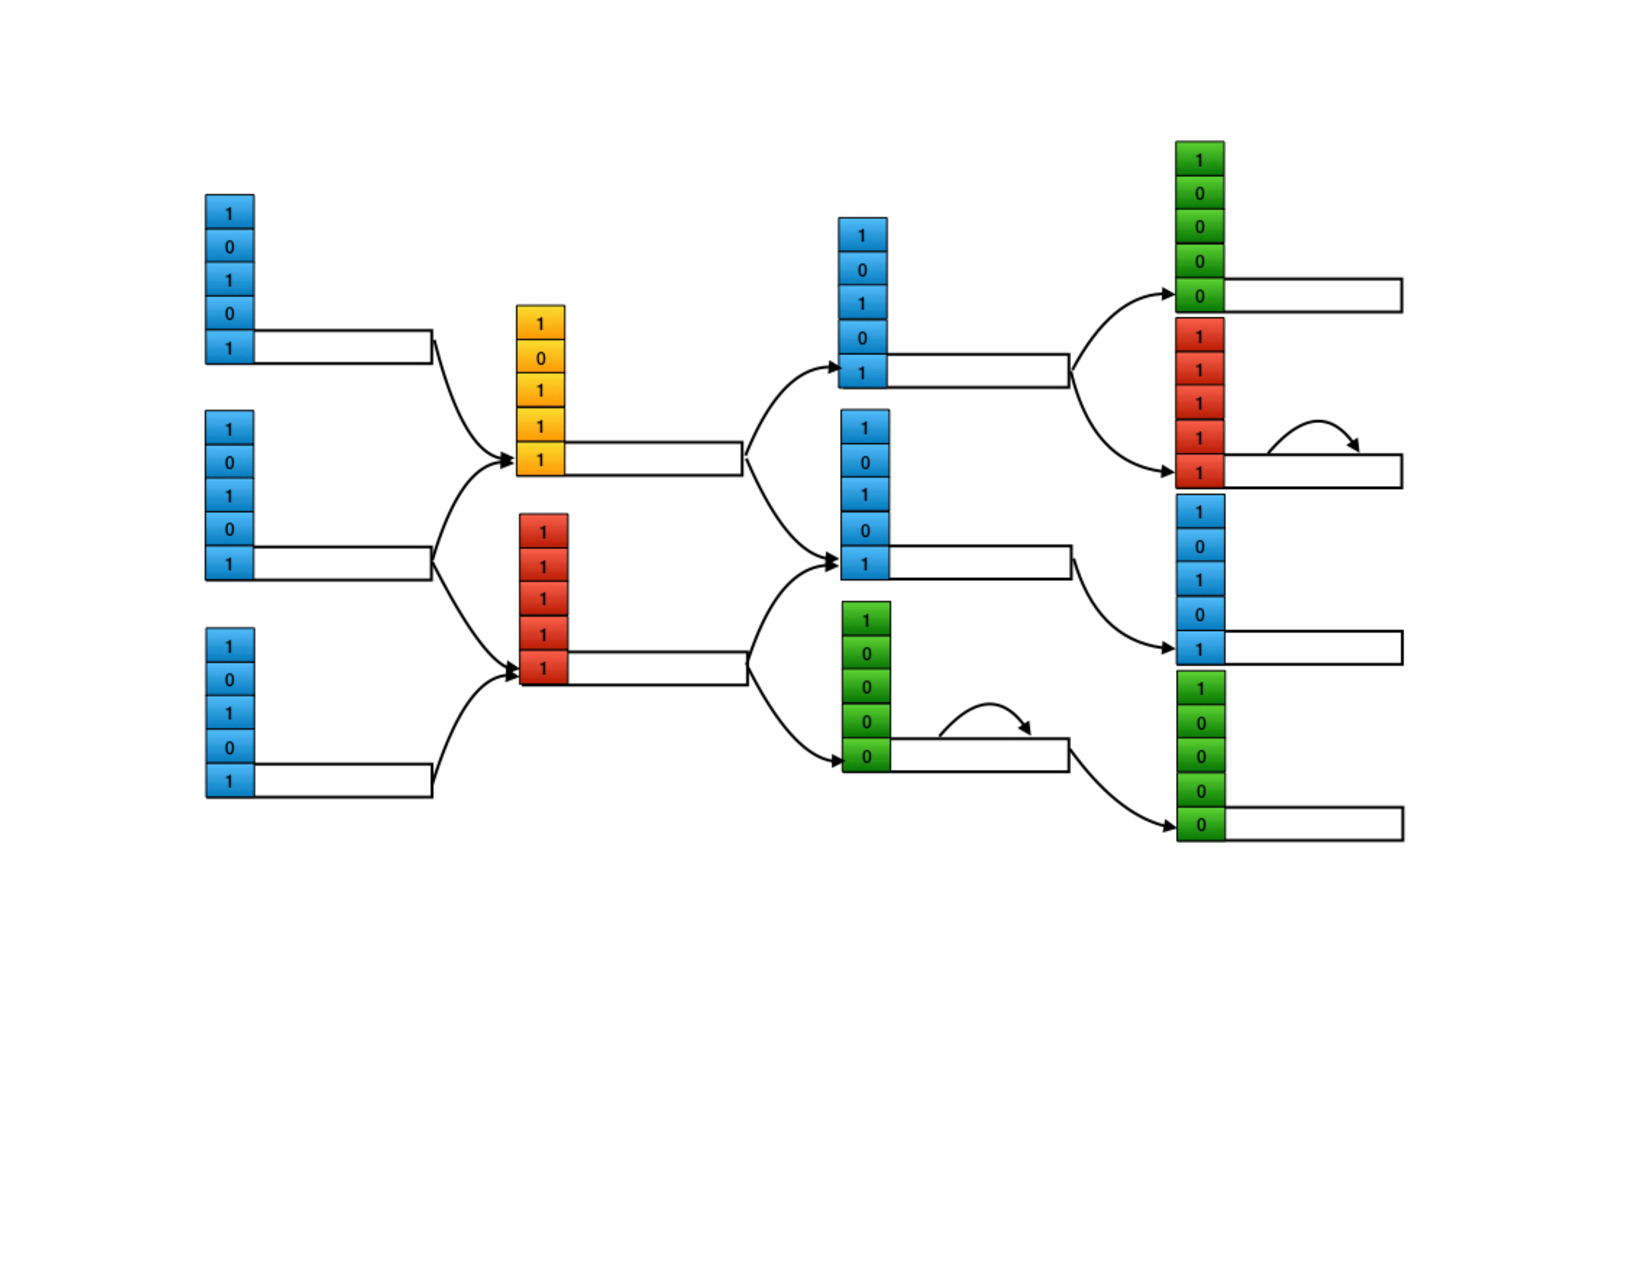
\includegraphics[width=0.7\columnwidth, trim={1in 2.5in 1.5in 1in},clip]{figs/mantis/cdbg}
        \caption{A colored de Bruijn graph.  Each rectangle node represents a \kmer.
        Each vector represents a color class (equal color classes have the same color).}
        \label{subfig-cdbg}
    \end{subfigure}%
    ~
    \begin{subfigure}[t]{0.49\textwidth}
        \captionsetup{width=0.7\columnwidth}
        \centering
        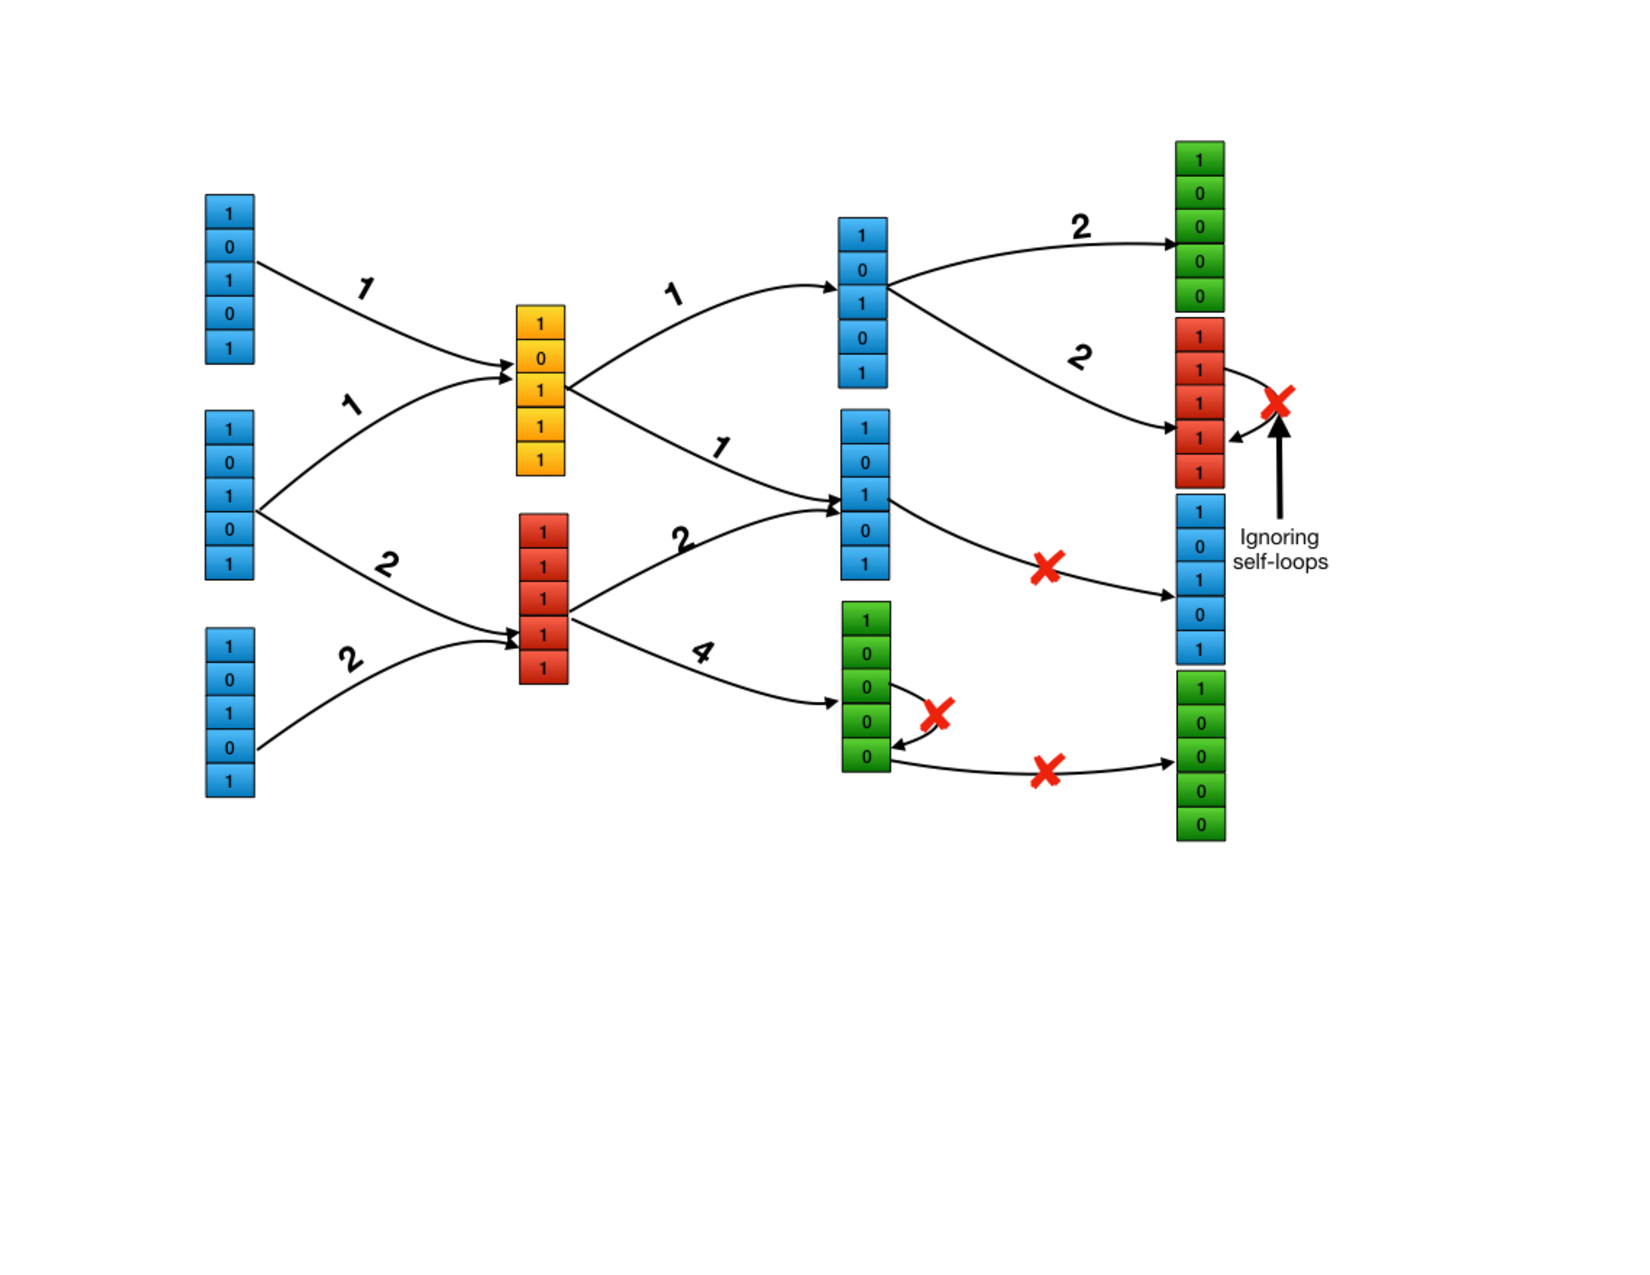
\includegraphics[width=0.7\columnwidth, trim={1in 2.5in 1.5in 1in},clip]{figs/mantis/cc}
        \caption{The \cc graph from the \cdbg. There is an edge between each pair of color classes
        that correspond to adjacent \kmers in \cdbg.
        Weights on the edges represent the Hamming distances of the \cc vectors.}
        \label{subfig-cc}
        \vspace{0.2in}
    \end{subfigure}
    ~

    \begin{subfigure}[t]{0.5\textwidth}
        \captionsetup{width=0.7\columnwidth}
        \centering
        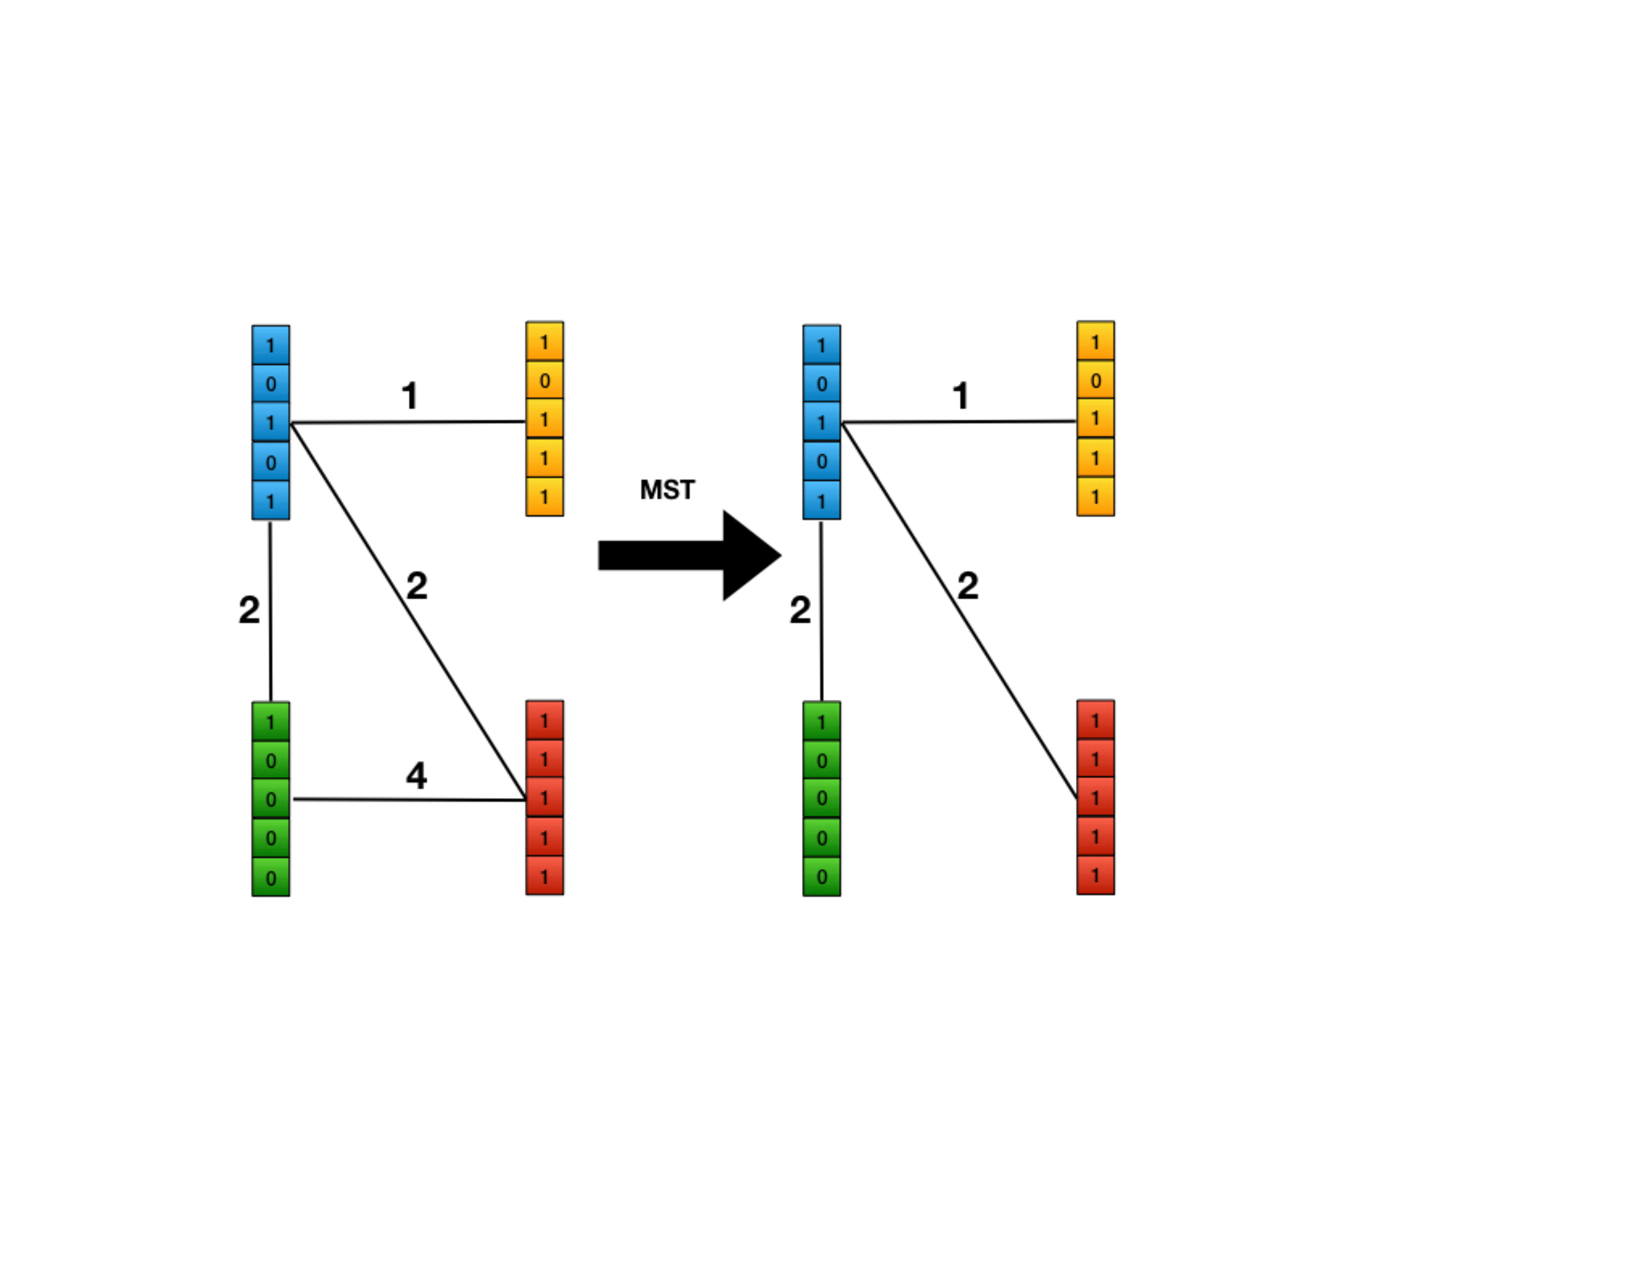
\includegraphics[width=0.7 \columnwidth, height=3.5cm, trim={1in 2in 2.5in 2in},clip]{figs/mantis/ourCg}
        \caption{The \cc graph we achieve from \ref{subfig-cc} by removing duplicate edges
        and its corresponding \mst.}
        \label{subfig-ourmst}
    \end{subfigure}%
    ~
    \begin{subfigure}[t]{0.5\textwidth}
        \captionsetup{width=0.7\columnwidth}
        \centering
        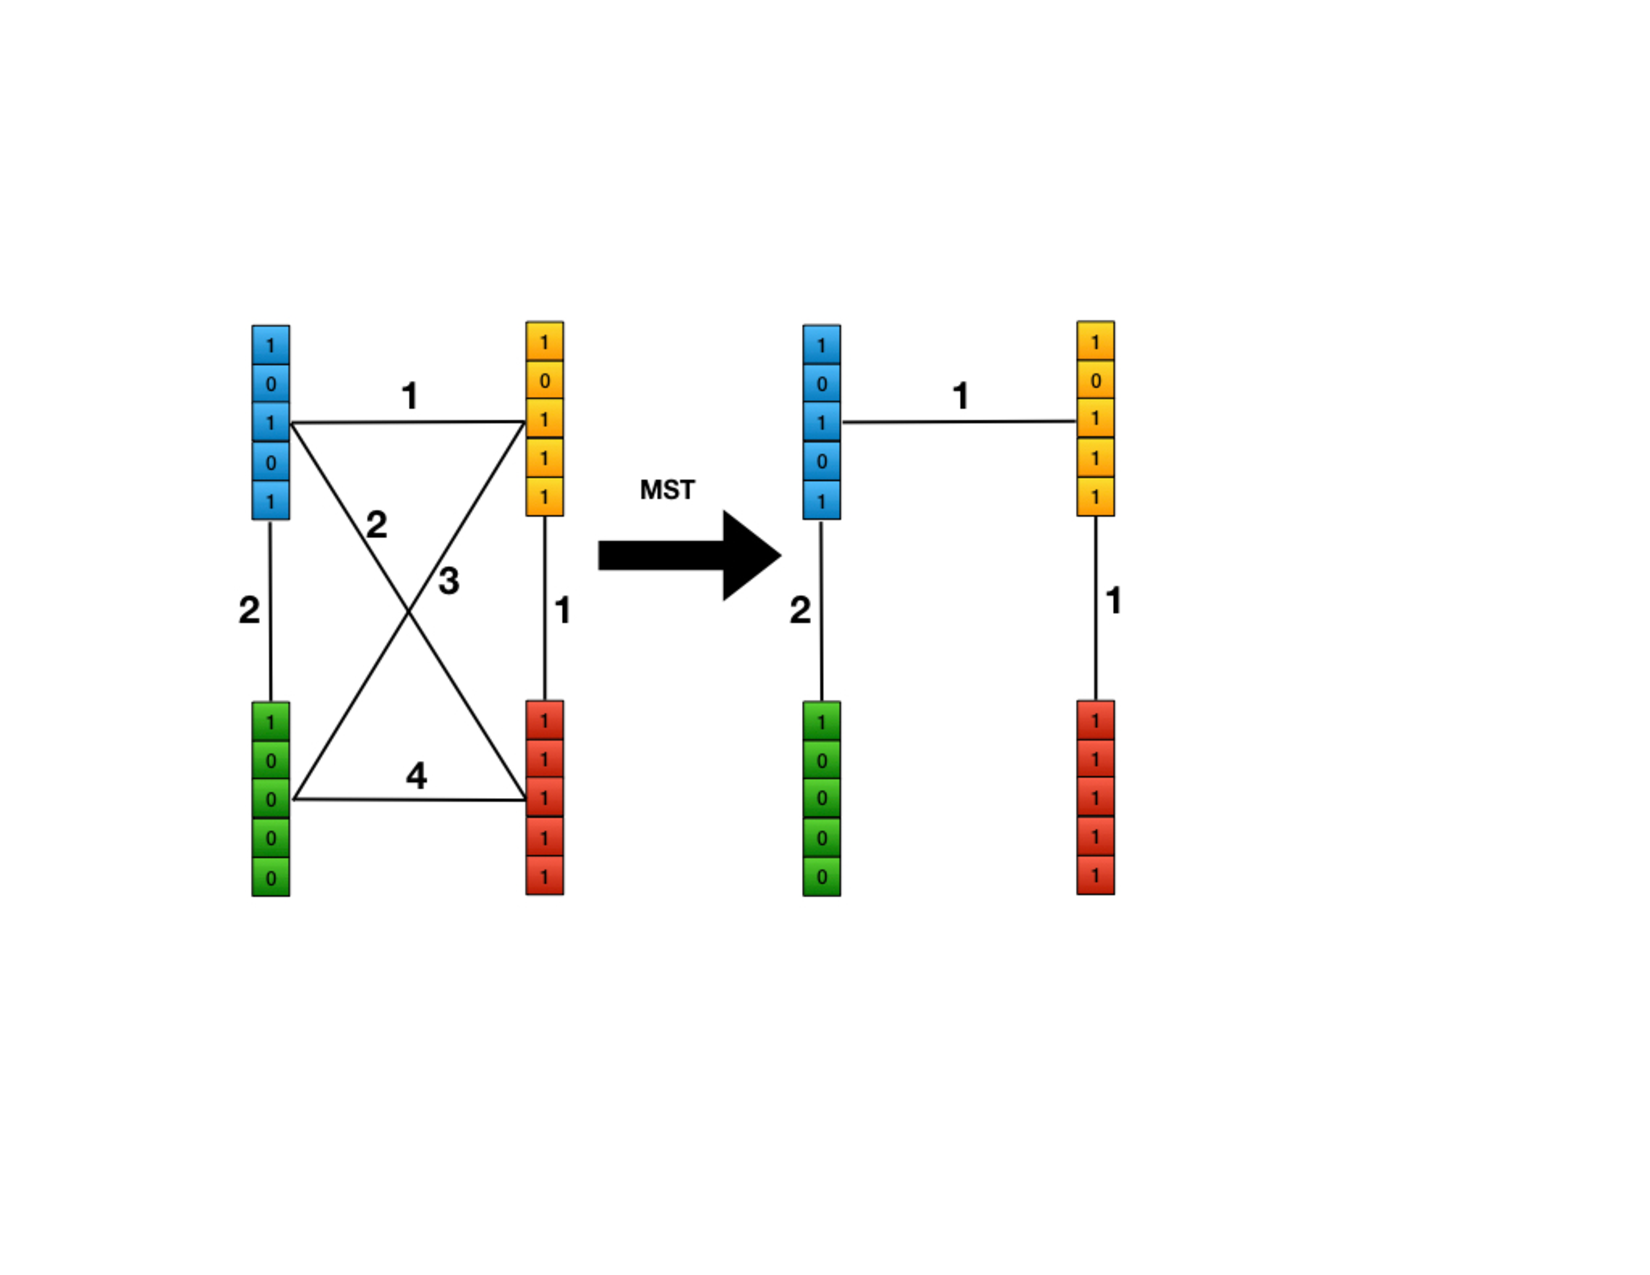
\includegraphics[width=0.7\columnwidth, height=3.5cm, trim={1in 2in 2.5in 2in},clip]{figs/mantis/optimalCg}
        \caption{The complete \cc graph
        and its derived \mst which has the minimum achievable total weight.}
        \label{subfig-optimalmst}
        \vspace{0.1in}
    \end{subfigure}
    \caption{Encoding \ccs by finding the \mst of the \cc graph, an undirected graph
    derived from \cdbg.
    The order of the process is \ref{subfig-cdbg}, \ref{subfig-cc},
    and \ref{subfig-ourmst}. The arrows in \ref{subfig-cdbg} and \ref{subfig-cc}
    show the direction of edges in the \dbg which is a directed graph. The optimal achievable
    \mst is shown in \ref{subfig-optimalmst} for comparison.
    Since we never observe the edge between any \kmers from \ccs green and yellow in \cdbg,
    we won't have the edge between \ccs green and yellow and therefore, our final \mst
    is not equal to the best \mst we can get from a complete \cc graph.
    }
    \label{fig:mstConstruction}
\end{figure*}


\subsection{Implementation of the MST data structure}

Assuming we have $|\calC|$ \ccs,
$|U|$ colors, and an \mst with total weight of $w$ over the \cc graph,
we store all the information required to retrieve the original \cbv for each \cc ID
based on the \mst structure into three data structures:
\begin{itemize}
    \item \textbf{Parent vector}: This vector contains $|\calC|$
    slots, each of size $\ceil{\log_2 {\calC}}$.  The value stored
    in index $i$ represents the parent \cc ID of the \cc with index
    $i$ in the \mst.
    \item \textbf{Delta vector}: This vector contains $w$ slots, each
    of size $\ceil{\log_2 {|U|}}$.  For each pair of parent and
    child in the parent vector, we compute a vector of the indices
    at which they differ.  The delta vector is the concatenation of
    these per-edge delta vectors, ordered by the ID of the source of
    the edge.  Note that the per-edge delta vectors will not all be
    of the same length, because some edges have larger weight than
    others.  Thus, we need an auxiliary data structure to record the
    boundaries between the per-edge deltas within the overall delta
    vector.
    %%   store the indices of the bits that are
    %% different between parent and child \cbvs. We call these different indices deltas of the two
    %% \cbvs. The order of the delta sets is the same as the order of the nodes in the \pbv.
    %    meaning that
    %     assuming $i \leq j$ be the indices of two child nodes in parent int-vector, the delta set
    %     for node $i$ and its parent comes before the delta set for node $j$ and its parent.
    \item \textbf{Boundary bit-vector}: This vector contains $w$ bits,
    where a set bit indicates the boundary between two delta sets
    within the delta vector.  To find the starting position, within
    the delta vector, of the per-edge delta list for the MST edge
    with source ID $i$, we perform \textit{select($i$)} on
    the boundary vector.  Select returns the position of the $i$th
    one in the boundary vector.
    %% For finding the deltas for a child at
    %% index $i$ in the parent vector and its parent, we use the
    %% succinct operation \textit{select} for index $i$ on the boundary
    %% bit-vector to find out the starting index of the delta set for
    %% $i$ in the delta int-vector.
\end{itemize}

\paragraph{Query of the \mst-based representation.} \Cref{fig:query} shows how queries proceed using this encoding.
We start with an empty accumulator bit vector and a color class ID $i$
for which we want to compute the corresponding color class.  We
perform a select query for $i$ and $i+1$ in the boundary bit-vector to get the
boundaries of $i$'s difference list in the delta vector.  We then
iterate over its difference list and flip the indicated bits in our
accumulator.  We then set $i\gets \textsc{parent}[i]$ and repeat
until $i$ becomes 0, which indicates that we have reached the root.
At this point, the accumulator will be equal to the bit vector for
color class $i$.

\begin{figure*}[t!]
    \centering
    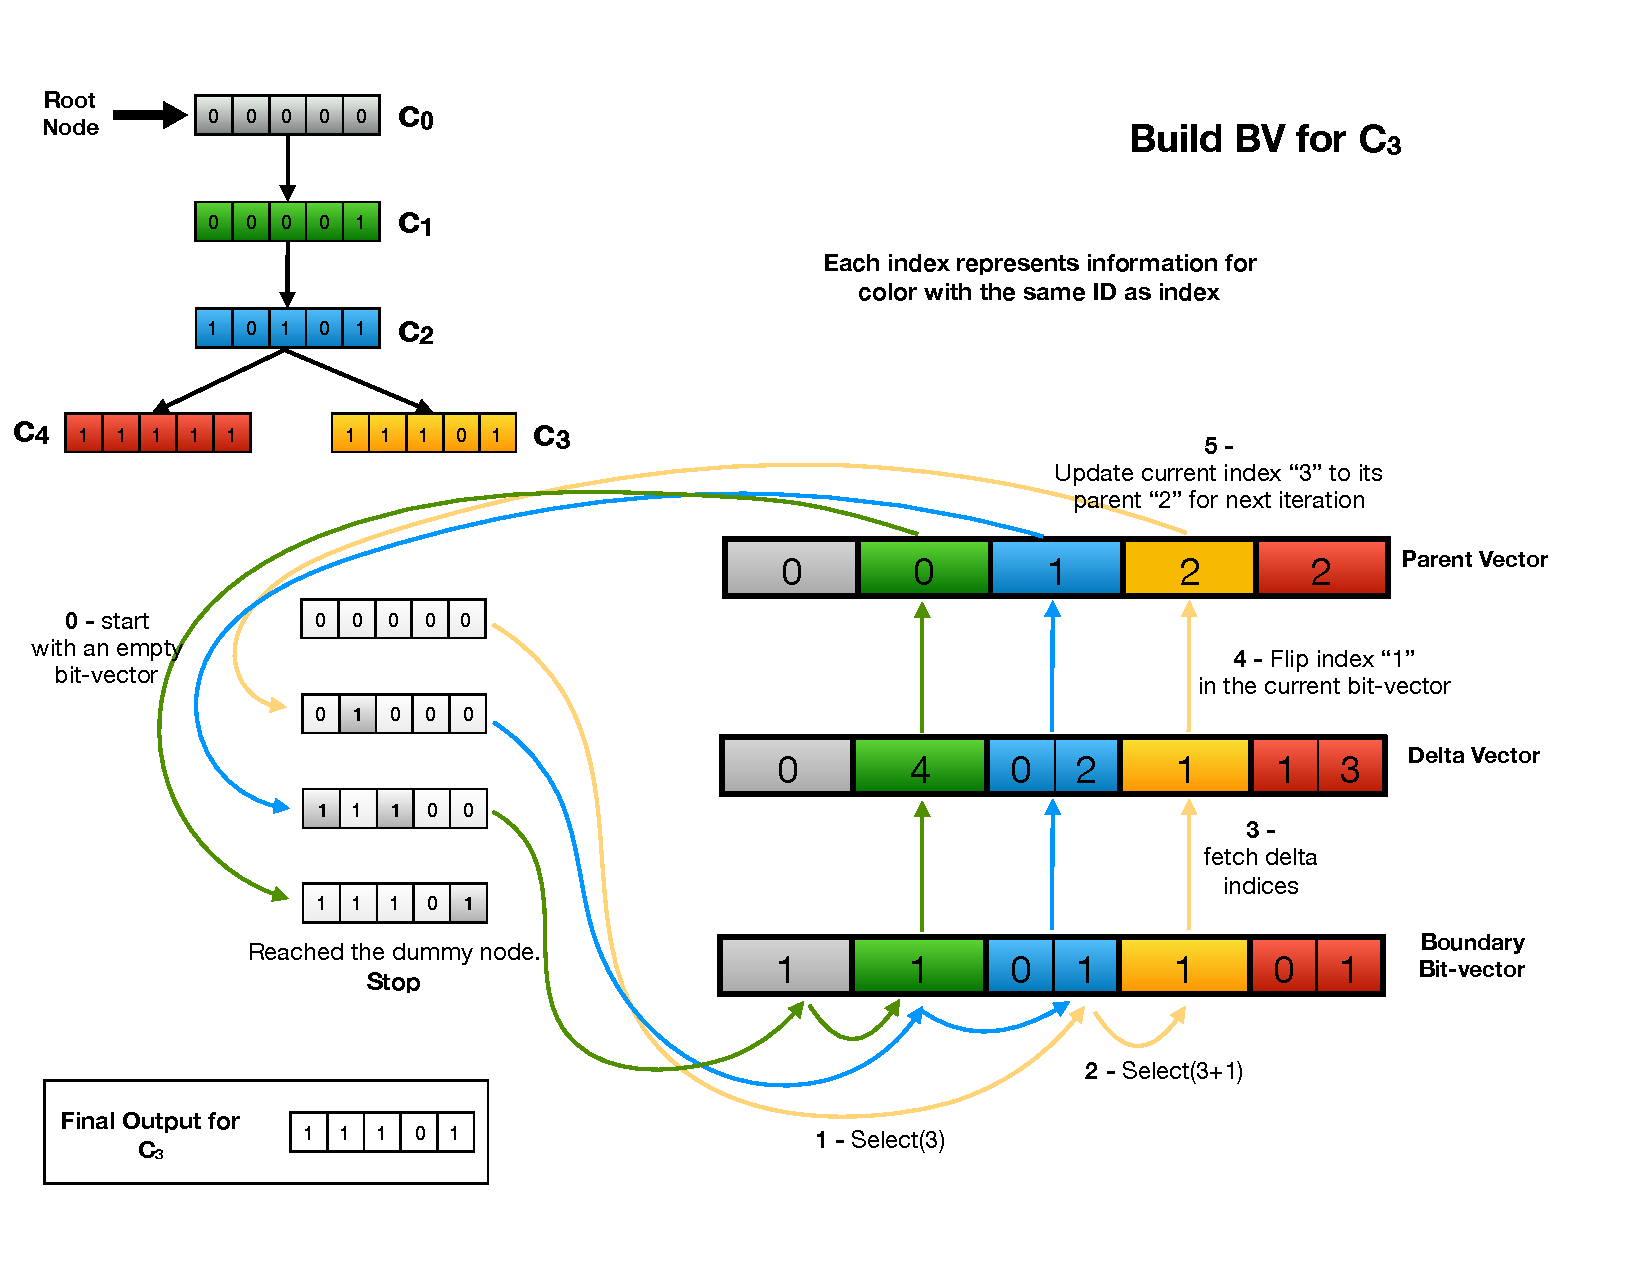
\includegraphics[width=0.65\columnwidth]{figs/mantis/figure2}
    \caption{The conceptual \mst (top-left), the data structure to
    store the color information in the format of an \mst (right).
    This figure also illustrates the steps required to build one of the color vectors ($C_3$) at the leaf
    of the tree. Note that the query process shown here does not depict the caching policy we apply in practice.}
    \label{fig:query}
    \vspace{-1.5em}
\end{figure*}


\subsection{Integration in Mantis}

Once constructed, our MST-based color class representation is a
drop-in replacement for the current color class representations used in
several existing tools, including Mantis~\cite{mantis} and
Rainbowfish~\cite{rainbowfish}.  Their existing color class
tables support a single operation---querying for a color class
by its ID---and our MST-based representation supports exactly
the same operation.

For this paper, we integrated our MST-based representation into
Mantis.  The same space savings can be achieved in
other tools, particularly Rainbowfish, which has
a similar color-class encoding as Mantis.

\ourparagraph{Construction.}
We construct our MST-based color-class representation as follows.
First, we run Mantis to build its default representation of the \cdbg.
We then build the color-class graph by walking the \dbg and adding all
the corresponding edges to the color-class graph.  The edge set is
typically much smaller than the \dbg (because many \dbg edges may map to
the same edge in the color-class graph), so this can be done in RAM.
Note that we do not compute the weights of the edges during this pass,
because that would require having all of the large color-class bit vectors
in memory in order to compute their Hamming distance.
%walk the \cdbg to determine which distinct colors are adjacent
%in the underlying \dbg.  This provides us with an edge set for our
%color graph.

In the second pass, we traverse the edge set and compute the weight of
each edge.  To minimize RAM usage during this phase, we sort
the edges and iterate over them in a ``blocked'' fashion.
Specifically, Mantis stores the color class bit vectors on-disk
sequentially by ID, grouped into blocks of roughly 6GBs each.  We sort
the edges lexicographically by their source and destination block. We then load
all pairs of blocks and compute the weights of all the edges between the two
blocks currently in memory. At all times, we need only two blocks of color class
vectors in memory. Given the weighted graph, we compute the \mst and make one
final pass to determine the relevant delta lists and encode our final \mst
structure.

\ourparagraph{Parallelization.}  We note that, after having
constructed the \mantis representation, most phases of the MST
construction algorithm are trivially parallelized.  MST construction
decomposes into three phases: (1) color-class graph construction, (2)
MST computation, and (3) color-class representation generation.
We parallelize graph construction and color-class representation
generation. The MST computation itself is not parallelized.

We parallelized the determination of edges in the color-class graph by
assigning each thread a range of the \kmer-to-color-class-ID
map. Each thread explores the neighbors of the \kmers that appear in
its assigned range, and any redundant edges are deduplicated when all
threads are finished.  Similarly, we parallelized the computation of
edge weights and the extraction of the delta vectors that correspond
to each edge in the MST. Given the list of edges sorted
lexicographically by their endpoints (determined during the first
phase), it is straightforward to partition the work for processing
batches of edges across many threads. It is possible, of course, that
the batches will display different workloads and that some threads
will complete their assigned work before others.  We have not yet made
any attempt to optimize the parallel construction of the MST in this
regard, though many such optimizations are likely possible.

\ourparagraph{Accelerating queries with caching.}
The encoded \mst is not a balanced tree, so decoding a \cbv might require
walking a long path to the root, which negatively impacts the query time.
Attempting to explicitly minimize the depth or diameter of the MST is, as
discussed in~\Cref{sec:intro}, not generally approximable within a constant
factor. However, considering the fact that the frequency distribution of
the \ccs is very skewed, some of the \ccs are more popular or have more children
and, therefore, are in the path of many more nodes. We take advantage of these
data characteristics by caching the most recent queried \cbvs. Every time we
walk up the tree, if the \cbv for a node is already in the cache, our query
algorithm stops at that point and applies all the deltas to this \bv instead of
the zero \bv of the root. This caching approach significantly improves the query
time, resulting in the final query time required to decode a \cc being
marginally faster than direct RRR access.

The cache policy is designed with the tree structure of our
color-class representation in mind.  Specifically, we want to cache
nodes near the leaves, but not so close to the leaves that we end up
caching essentially the entire tree.  Also, we don't want to cache
infrequently queried nodes.  Thus we use the following caching policy:
all queried nodes are cached.  Furthermore, we cache interior nodes
visited during a query as follows.  If a query visits a node that
has been visited by more than 10 other queries and is more than
10 hops away from the currently queried item, then we add that node
to the cache.  If a query visits more than one such node, we add
the first one encountered.

In our experiments, we used a cache of 10,000 nodes and managed the
cache using a FIFO policy.

\subsection{Comparison with brute-force and approximate-nearest-neighbor-based approaches}

Our MST-based color-class representation uses the \dbg as a hint as to
which color classes are likely to be similar.  This leads to the
natural question: how good are the hints provided by the \dbg?

One could imagine alternatively constructing the MST on the complete
color-class graph.  This would yield the absolutely lowest-weight
spanning tree on the color classes.  Unfortunately, no MST algorithm
runs in less than $\Omega(|E|)$ time, so this would make our
construction time quadratic in the number of color classes.  The
number of color classes in our experiments range from $10^{6}$ to
$10^9$, so the number of edges in the complete color-class graph would
be on the order of $10^{12}$ to $10^{18}$, or possibly even more,
making this algorithm impractical for the largest data sets considered
in this paper.

Alternatively, we could try to use an approximate nearest-neighbor
algorithm to find pairs of color classes with small Hamming distance.
As an experiment, we implemented an approximate nearest neighbor
algorithm that bucketed color classes by their projection into
a smaller-dimensional subspace.  Nearest-neighbor queries were
computed by searching within the queried item's bucket.
Results were disappointing.  Even on small data sets, the average
distance between the queried item and the returned neighbor
was several times larger than the average distance found using
the neighbors suggested by the \dbg.  Thus, we did not pursue
this direction further.

%%%%%%%%%%%%%%%%%%%%%%%%%%%%%%%%%%%%%%%%%%%%%%%%%%%%%%%%%%%%
%%
%% Results section
%%
%%%%%%%%%%%%%%%%%%%%%%%%%%%%%%%%%%%%%%%%%%%%%%%%%%%%%%%%%%%%
\section{Evaluation}
\label{sec:mantis_eval}

In this section we evaluate our MST-based representation of the color
information in the \cdbg.  All our experiments use Mantis with
our integrated MST-based color-class representation.


\ourparagraph{Evaluation Metrics}
We evaluate our MST-based representation on the following parameters:
\begin{itemize}
    \item \textbf{Scalability.} How does our MST-based color-class representation
    scale in terms of space with increasing number of input samples, and how does
    it compare to the existing representations of \mantis?

    \item \textbf{Construction time.} How long does it take --- in addition to
    the original construction time for building \cdbg --- to build
    our MST-based color-class representation?

    \item \textbf{Query performance.} How long does it takes to query the \cdbg
    using our MST-based color-class representation?
\end{itemize}
\subsection{Experimental procedure}

\label{experimental-proc}

\ourparagraph{System Specifications}

Mantis takes as input a collection of \defn{squeakr} files~\cite{PandeyBeJo17}.
Squeakr is a \kmer counter that takes as input a collection of fastq
files and produces as output, a single file with a compact hash table
mapping each \kmer to the number of times it occurs in the input
files.  As is standard in evaluations of large-scale sequence search indexes,
we do not benchmark the time required to construct these filters.

The data input to the construction process
was stored on 4-disk mirrors (8 disks
total).  Each is a Seagate 7200rpm 8TB disk (ST8000VN0022). They were formatted
using ZFS and exported via NFS over a 10Gb link.
We used different systems to run and evaluate time, memory,
and disk requirements for the two steps of preprocessing and
index building as was done by~\citet{mantis}.

For index building and query benchmarks, we ran all the experiments on
the same system used in \mantis~\citep{mantis}, an
Intel(R) Xeon(R) CPU (E5-2699 v4 @2.20GHz with 44 cores and 56MB L3 cache) with
512GB RAM and a 4TB TOSHIBA MG03ACA4 ATA HDD running Ubuntu 16.10 (Linux kernel
4.8.0-59-generic).  Constructing the main index was done using a single thread,
and the MST construction was performed using $16$ threads.  Query benchmarks
were also performed using a single thread.

% Explaining the 10,000 experiments
\ourparagraph{Data to evaluate scalability and comparison to \mantis}

We integrated and evaluated our MST-based color-class representation
within Mantis, so we briefly review Mantis here. Mantis builds an index on a
collection of unassembled raw sequencing data sets. Each data set is called a
\defn{sample}. The Mantis index enables fast queries of the form, ``Which
samples contain this \kmer,'' and ``Which samples are likely to contain this
string of bases?'' Mantis takes as input one \defn{squeakr} file per
sample~\cite{PandeyBeJo17}. A squeakr file is a compact hash table mapping each
\kmer to the number of times it occurs within that sample. \squeakr also has the
ability to serialize a hash that simply represents the set of \kmers present at
or above some user-provided threshold; we refer to these as filtered \squeakr
files. Using the filtered \squeakr files vastly reduces the required
intermediate storage space, and also decreases the construction time required
for Mantis considerably. For example, for the breast, blood, and brain dataset
($2586$ samples), the unfiltered \squeakr files required $\sim2.5$TB of space
while the filtered files require only $\sim108$GB. To save intermediate storage
space and speed index construction, we built our Mantis representation from
these filtered \squeakr files.


Given the input files, Mantis constructs an index consisting of two
files: a map from \kmer to color-class ID, and a map from color-class
ID to the bit vector encoding that color class.  The first map is
stored as a \defn{counting quotient filter} (CQF), which is the same
compact hash table used by Squeakr.  The color-class map is an
RRR-compressed bit vector.

Recall that our construction process is implemented as a
post-processing step on the standard Mantis color-class
representation.  For construction times, we report only this
post-processing step.  This is because our MST-based color-class
representation is a generic tool that can be applied to many \cdbg
representations other than Mantis, so we want to isolate the time
spent on MST construction.

To test the scalability of our new \cc representation, we used a
randomly-selected set of $10,000$ paired-end, human, bulk RNA-seq short-read
experiments downloaded from European Nucleotide Archive(ENA)~\citep{nih-sra} in
gzipped FASTQ format. Additionally, we have built the proposed index for
$2,586$ sequencing samples from human blood, brain, and breast tissues (\bbb)
originally used by~\cite{Solomon2016Fast} and also used in the subsequent
work~\citep{Solomon2017Improved,Sun2017Allsome,seqothello}, including
\mantis~\citep{mantis}, as a point of comparison with these representations.
The set of $10,000$ experiments does not overlap with the \bbb samples.
The full list of $10,000$ experimental identifiers can be obtained from
\url{https://github.com/COMBINE-lab/color-mst/blob/master/input_lists/nobbb10k_shuffled.lst}.
%\url{https://github.com/COMBINE-lab/color-mst/blob/master/input_lists/shuffled_10k_paired}.
The total size of all these experiments (gzipped) is $25.23$TB.
%new result: 27745362006992%%%old result: 27550806707164%

% Cutoffs
In order to eliminate spurious \kmers that
occur with insignificant abundance within a sample, the squeakr files
are filtered to remove low-abundance \kmers.
We adopted the same cutoff policy originally proposed by~\citet{Solomon2016Fast},
by discarding \kmers that occur less than some threshold number of time.  The
thresholds are determined according to the size (in bytes) of the gzipped
sample, and the thresholds are given in \Cref{tab:cutoffs}.  We adopt a value of
$k=23$ for all experiments.
\begin{table}[t]
    \centering
    \begin{tabular}{r@{\hskip 0.5in}r@{\hskip 0.5in}r@{\hskip 0.5in}c}
        \hline
        Min size & Max size    & Cutoff & \begin{tabular}{c}\# of experiments \\ with specified threshold\end{tabular}\\
        \hline
        \hline
        0        & $\leq 300$MB   & 1  & 2,784\\
        $>300$MB & $\leq 500$MB   & 3  & 798\\
        $>500$MB & $\leq 1$GB     & 10 & 1,258\\
        $>1$GB   & $\leq 3$GB     & 20 & 2,296\\
        $>3$GB   & $\infty$       & 50 & 2,864\\
        \hline
    \end{tabular}
    \caption{\label{tab:cutoffs}Minimum number of times a \kmer must
    appear in an experiment in order to be counted as abundantly
    represented in that experiment (taken from the SBT paper). Note,
    the \kmers with count of ``cutoff'' \emph{are} included at each
    threshold.}
    \vspace{-2.5em}
\end{table}

\subsection{Evaluation results}

\ourparagraph{Scalability of the new \cc representation}
\Cref{fig:scaling} and \Cref{tab:growthrate} show how the size of our
MST-based color-class representation scales as we increase the number
of samples indexed by Mantis.  For comparison, we also give the size
of Mantis' RRR-compression-based color-class representation.
\Cref{fig:scaling} also plots the size of the CQF that Mantis uses to
map \kmers to color class IDs. We can draw several conclusions from this data:
\begin{itemize}
    \item {The MST-based representation is an order-of-magnitude
    smaller than the RRR-based representation.}
    \item {The gap between the RRR-based representation and the
    MST-based representation grows as we increase the number of input
    samples.}  This suggests that the MST-based representation
    grows asymptotically slower than the RRR-based representation.
    \item {The MST-based color-class representation is, for large
    numbers of samples, about 5$\times$ smaller than the CQF.}  This
    means that representing the color classes is no longer the scaling
    bottleneck.
\end{itemize}

\begin{figure*}[t!]
    %    \captionsetup[subfigure]{justification=centering}
    \centering
    \begin{subfigure}[t]{3in}
        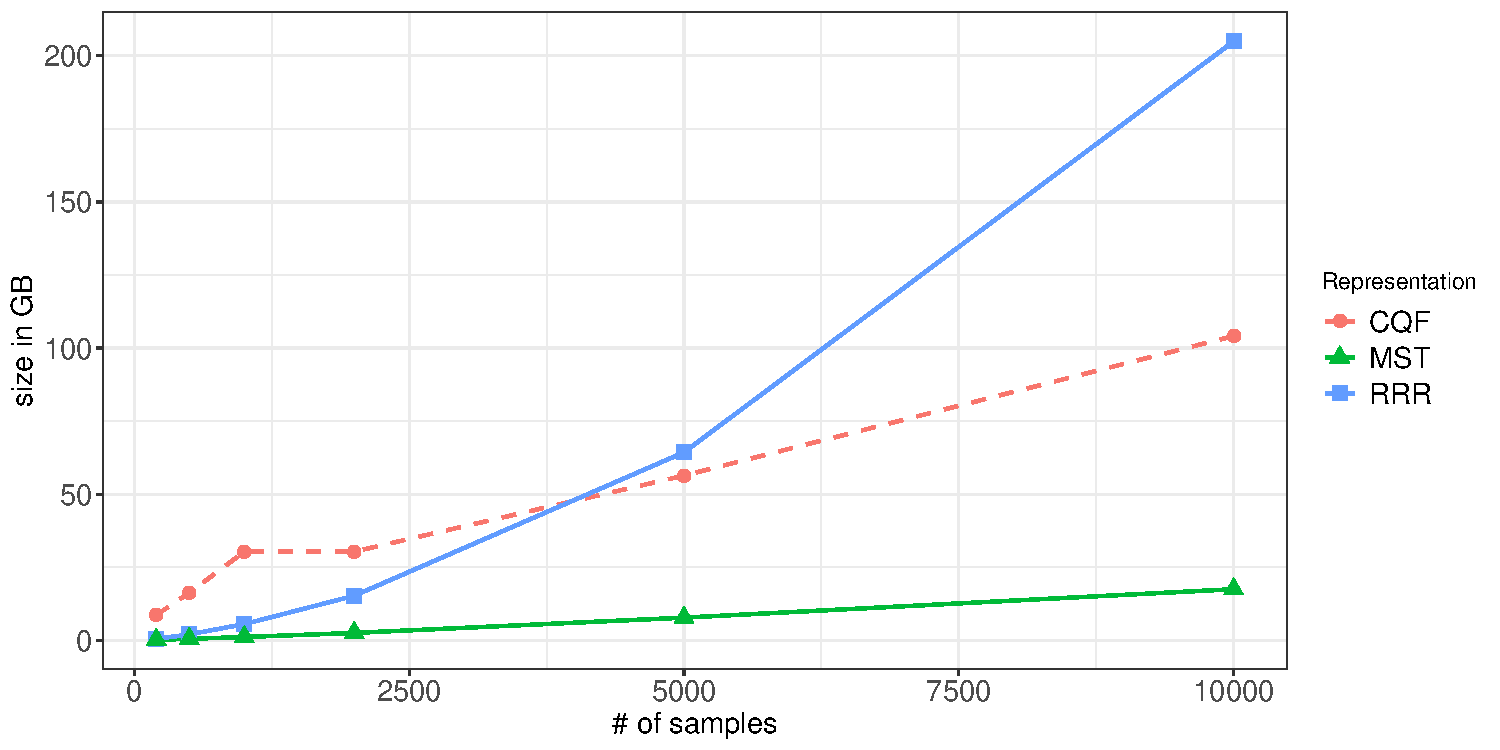
\includegraphics[width=3in]{figs/mantis/scaling_r2}
        \caption{Sizes of the RRR and \mst-based \cc representations with
        respect to the number of samples indexed from the human bulk RNA-seq data set.
        The \cqf component is the Mantis representation of the \dbg.}
        \label{fig:scaling}
    \end{subfigure}
    ~~~~~~~~~~~
    \begin{subfigure}[t]{3in}
        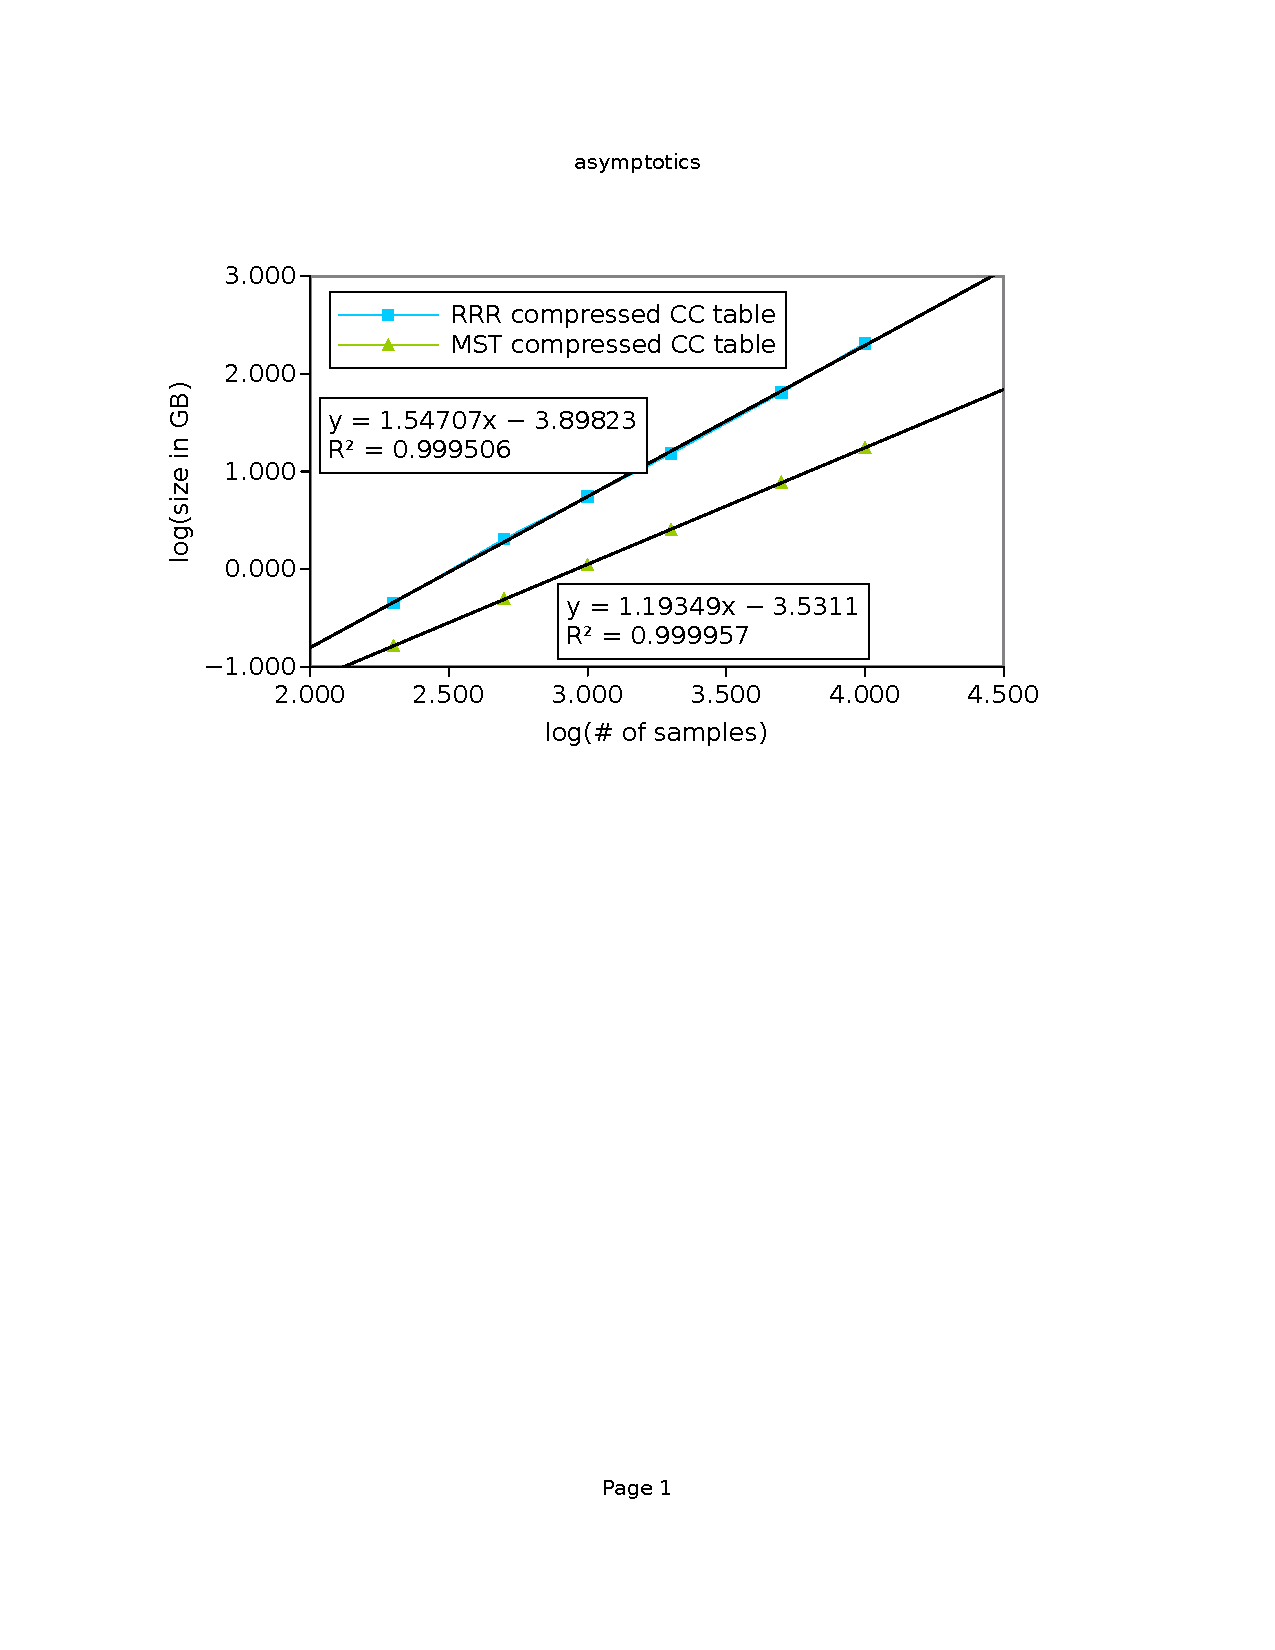
\includegraphics[width=3in,clip, trim = 1.1in 6in 1.5in 1.75in]{figs/mantis/asymptotics__asymptotics}
        \caption{Empirical asymptotic analysis of the growth rates of the
        sizes of RRR-based \cc representation and the MST-based
        \cc representation.  The RRR-based representation grows
        at a rate of $\approx \Theta(n^{1.5})$, where $n$ is the number of
        samples.  The MST-based representation grows at a rate of
        $\approx\Theta(n^{1.2})$.}
        \label{fig:asymptotics}
        \vspace{.1in}
    \end{subfigure}
    \caption{Size of the MST-based color-class representation vs.
    the RRR-based color-class representation.}
\end{figure*}

\Cref{tab:growthrate} also shows the scaling rate of all elements of
the \mst representation, in addition to the ratio of \mst over the
\cbv.  As expected, the list of deltas dominate the \mst
representation both in terms of total size and in terms of
growth. \Cref{tab:growthrate} also shows the average edge weight of
the edges in the \mst.  The edge weight grows approximately
proportional to $\Theta(\log(\text{\# of samples}))$ (i.e., every time
we double the number of samples, the average edge weight increases by
almost exactly 1). This suggests that our \dbg-based algorithm
is able to find pairs of similar color classes. The time column shows the time
required to build the \mst representation (which is in addition to the \mantis
construction time required to produce the input to the \mst compression
algorithm).

To better understand the scaling of the different components of a
\cdbg representation, we plot the sizes of the RRR-based color-class
representations and MST-based representations on a log-log scale in
\Cref{fig:asymptotics}. Based on the data, the RRR-based
representation appears to grow in size at a rate of roughly
$\Theta(n^{1.5})$, whereas the new MST-based representation grows
roughly at a rate of $\Theta(n^{1.2})$. This explains why the
RRR-based representation grows to dwarf the CQF (which grows roughly
linearly) and become the bottleneck to scaling to larger data sets,
whereas the MST-based representation does not. With the MST-based
representation, the CQF itself is now the bottleneck.

Finally, the last two rows in \Cref{tab:growthrate} show the size of the RRR- and MST-based
color-class representations for the human blood, brain, breast (\bbb) and \textit{E. coli} data sets respectively.
\bbb is the data set used in \sbt and
its subsequent tools~\citep{Solomon2017Improved,Sun2017Allsome,seqothello},
as well as in \mantis~\citep{mantis}
and \textit{E. coli} is the data set analyzed in the Rainbowfish paper.
This dataset, which has been obtained from
GenBank~\cite{o2015reference}, consists of $5,598$ distinct \emph{E. coli}
strains. Since the strain assemblies are all from the same species,
\emph{E. coli}, each strain shares a large portion of its sequence with the others.
We specifically chose this dataset since \rainbowfish has already
demonstrated a large improvement in size for it compared to
Vari~\citep{MuggliBoNo17}.

As the table shows, our MST-based
color-class representation is able to effectively compress genomic
color data in addition to RNA-seq color data.

\begin{table}[t]
    \centering
    \resizebox{\columnwidth}{!}{%
    \begin{tabular}{c|c@{\hskip 0.05in}c@{\hskip 0.05in}c@{\hskip 0.05in}c
    @{\hskip 0.05in}c@{\hskip 0.05in}c@{\hskip 0.05in}c@{\hskip 0.05in}c
    @{\hskip 0.15in}c@{\hskip 0.15in}c}
        \hline
        & & & \multicolumn{4}{c}{MST} \\ \cline{4-9}
        \multicolumn{1}{p{1.5cm}|}{\centering Dataset}
        & \multicolumn{1}{p{1.5cm}}{\centering \# samples}
        & \multicolumn{1}{p{1.5cm}}{\centering RRR matrix}
        & \multicolumn{1}{p{1.5cm}}{\centering Total \\ space}
        & \multicolumn{1}{p{1.5cm}}{\centering Parent \\ vector}
        & \multicolumn{1}{p{1.5cm}}{\centering Delta \\ vector}
        & \multicolumn{1}{p{1.5cm}}{\centering Boundary \\ bit-vector}
        %     & \multicolumn{1}{p{1.5cm}}{\centering Build \\ memory \\ (GB)}
        & \multicolumn{1}{p{1.5cm}}{\centering Build \\ time \\ (hh:mm:ss)}
        & \multicolumn{1}{p{1.5cm}}{\centering Expected \\ edge weight}
        & \multicolumn{1}{p{1.5cm}}{\centering $\frac{\text{size}(\mst)}{\text{size}(\text{RRR})}$}
        \\
        %& $\frac{weight(\mst)}{count(edges)}$ \\
        \hline
        \hline
        \multirow{6}{*}{\begin{tabular}{c}\textit{H. sapiens} \\ RNA-seq \\ samples\end{tabular}}
        & 200    & 0.42 & 0.15 & 0.08 & 0.06 & 0.01 & 0:05:42 & 2.42 & 0.37   \\ % mst/cbv: 68050395/28923216
        & 500    & 1.89 & 0.46	& 0.2 & 0.24	& 0.03	& 0:12:15 & 3.42 & 0.24  \\ % mst/cbv: 213655826/62036089
        & 1,000  & 5.14 & 1.03 & 0.37 & 0.6 & 0.06 & 0:25:03 & 4.39 & 0.2   \\ % mst/cbv: 492089063/110586891
        & 2,000  & 14.2 & 2.35 & 0.71 & 1.5 & 0.14 & 0:51:58 & 5.38 & 0.17  \\ % mst/cbv: 1092711068/198418790
        & 5,000  & 59.89 & 7.21 & 1.72 & 5.1 & 0.39 & 3:52:34 & 6.61 & 0.12   \\ % mst/cbv: 3120503401/457178572
        & 10,000 & 190.89 & 16.28 & 3.37 & 12.06 & 0.86 & 10:17:42 & 7.68 & 0.085  \\ % mst/cbv: 6974169057/893128926
        \hline
        \begin{tabular}{c} Blood, Brain,\\Breast (\bbb) \end{tabular} & 2586 & 15.8 & 2.66 & 0.63 & 1.88 & 0.16 & 00:57:43 & 6.98 & 0.17 \\
        \hline
        \begin{tabular}{c}\textit{E. coli} strain \\ reference genomes\end{tabular} & 5,598 & 2.06 & 0.83 & 0.02 & 0.76 & 0.06 & 00:03:15 & 7.8 & 0.4 \\ % mst/cbv: 6974169057/893128926
        \hline
    \end{tabular}
    }
    \vspace{0.1in}
    \caption{Space required for RRR and \mst-based \cc encodings over different numbers of samples (sizes in GB)
    and time and memory required to build \mst. Central columns break down the size of individual \mst components.}
    \label{tab:growthrate}
    \vspace{-1em}
\end{table}

\begin{table}[t]
    \centering
    %\resizebox{\columnwidth}{!}{%
    \begin{tabular}{c|c@{\hskip 0.05in}c@{\hskip 0.05in}c}
        \hline
        \multicolumn{1}{p{1.5cm}|}{\centering Dataset}
        & \multicolumn{1}{p{1.5cm}}{\centering \# samples}
        & \multicolumn{1}{p{3cm}}{\centering Mantis Build memory (GB)}
        & \multicolumn{1}{p{2cm}}{\centering MST Build memory (GB)}
        \\
        \hline
        \hline
        \multirow{6}{*}{\begin{tabular}{c}\textit{H. sapiens} \\ RNA-seq \\ samples\end{tabular}}
        & 200    & 5 & 8 \\
        & 500    & 10 & 16 \\
        & 1,000  & 18 & 29 \\
        & 2,000  & 25 & 29 \\
        & 5,000  & 58 & 59 \\
        & 10,000 & 111 & 111 \\
        \hline
        \begin{tabular}{c} Blood, Brain,\\Breast (\bbb) \end{tabular} & 2586 & 28 & 29 \\
        \hline
        %\begin{tabular}{c}\textit{E. coli} strain \\ reference genomes\end{tabular} & 5,598 & 4?? & 6 \\
        %\hline
    \end{tabular}
    \vspace{0.1in}
    \caption{The memory required for \mantis build and \mst compression phases on
    human RNA-seq data. The overall memory required to construct the full index
    is the max of the two columns which, for these datasets, is always the \mst memory.}
    \label{tab:memory}
    \vspace{-1em}
\end{table}


\ourparagraph{Index Building Evaluation}
% Preprocessing
%Both tools \system and \seqothello have a preprocessing part before building the final index.
The ``Build time'' column in \Cref{tab:growthrate}
%\Cref{fig:mst-building-benchmark}
shows the time required to build our
MST-based color-class representation from Mantis' RRR-based
representation. All builds used 16 threads.
\Cref{tab:paraBenchmarks} shows how the \mst construction time for a $1000$
sample dataset scales as a function of the number of build threads. The memory
consumption is not affected by number of threads and remains fixed for all
trials.
The memory usage for both the main \mantis build and the \mst
construction steps is shown in \Cref{tab:memory}. Since these phases are run
independently, and since the \mst phase follows the \mantis construction phase, the
peak memory for the whole build pipeline is the maximum of the memory required
for each of the two construction phases.


\begin{table}[t]
    \centering
    \begin{tabular}{r||@{\hskip 0.3in}c@{\hskip 0.3in}c@{\hskip 0.3in}c@{\hskip 0.3in}c@{\hskip 0.3in}c@{\hskip 0.3in}c}
        \hline
        \# of threads  & 1 & 2 & 4 & 8 & 16 & 32\\
        \hline
        Run time (hh:mm:ss) & 02:47:08 & 01:38:26 & 01:02:42 & 00:31:57 & 00:22:00 & 00:14:17\\
        \hline
    \end{tabular}
    \vspace{0.1in}
    \caption{\label{tab:paraBenchmarks} The \mst
    construction time for $1000$ experiments using
    different number of threads.
    Memory stays the same across all the runs.}
    \vspace{-2.5em}
\end{table}

Overall, the MST construction time is only a tiny fraction of the
overall time required to build the Mantis index from raw fastq files.
The vast bulk of the time is spent processing the fastq files to
produce filtered squeakrs.  This step was performed on a cluster
of 150 machines over roughly one week.  Thus MST construction
represents less than 1\% of the overall index build time. The memory required to
build the MST is dependent on the size of the CQF and grows proportional to
that. In fact, due to the multi-pass construction procedure, the peak MST
construction memory is essentially the size of the CQF plus a relatively small
(and adjustable) amount of working memory. For the run over $10k$ experiments,
where the CQF size was the largest ($98G$), the peak memory required to build MST
is $111G$.


\ourparagraph{Query Evaluation}
%
\begin{table}[t]
    \centering
    \begin{tabular}{l@{\hskip 0.2in}|c@{\hskip 0.2in}c@{\hskip 0.2in}c|c@{\hskip 0.2in}c@{\hskip 0.2in}c}
        \hline
        & \multicolumn{3}{c}{\mantis} & \multicolumn{3}{c}{\mantis} \\
        \hline
        \hline
        & index load $+$ query & query & space & index load $+$ query & query & space \\
        10 Transcripts & 1 min 10 sec & 0.3 sec & 118GB & 32 min 59 sec & 0.5 sec & 290GB \\
        100 Transcripts & 1 min 17 sec & 8 sec & 119GB & 34 min 33 sec & 11 sec & 290GB \\
        1000 Transcripts & 2 min 29 sec & 79 sec & 120GB & 46 min 4 sec & 80 sec & 290GB \\
        \hline
    \end{tabular}
    \vspace{0.1in}
    \caption{\label{tab:query-benchmark} Query time and resident memory for
    mantis using the \mst-based representation for color information and the
    original mantis (using RRR-compressed \ccs) over $10,000$ experiments. The
    ``query'' column provides just the time taken to execute all queries (as would
    be required if the index was already loaded in e.g. a server-based search
    tool). Note that, in resident memory usage for the \mst-based representation,
    the \cqf always dominates the total required memory.}
    \vspace{-3em}
\end{table}
%
We evaluate query speed in the following manner. We select random
subsets, of increasing size, of transcripts from the human
transcriptome, and query the Mantis index to determine the set of
experiments containing each of these transcripts.  Mantis answers
transcript queries as follows.  For each \kmer in the transcript, it
computes the set of samples containing that \kmer.  It then reports a
sample as containing a transcript if the sample contains more than
$\Theta$ fraction of the \kmers in the transcript, where $\Theta$ is a
user-adjustable parameter.  Note that, for Mantis, the $\Theta$
threshold is applied at the very end.  Mantis first computes, for each
sample, the fraction of \kmers that occur in that sample, and then
filters as a last step.  Thus the query times reported here are valid
for any $\Theta$.

\Cref{tab:query-benchmark} reports the query performance of both the RRR
and \mst-based Mantis indexes. Despite the vastly-reduced space occupied by the
\mst-based index, and the fact that the \cc decoding procedure is more involved,
query in the MST-based index is slightly faster than querying in the RRR-based index.
The average query time in both RRR-based and \mst-based index
is $0.08$ sec / query.

Once the index has been loaded into RAM, Mantis queries are much faster than the
three \sbt-based large-scale sequence search data structures, and our MST-based
color-class representation doesn't change that.

%
%%%%%%%%%%%%%%%%%%%%%%%%%%%%%%%%%%%%%%%%%%%%%%%%%%%%%%%%%%%%
%%
%% Discussion!!!
%%
%%%%%%%%%%%%%%%%%%%%%%%%%%%%%%%%%%%%%%%%%%%%%%%%%%%%%%%%%%%%
\section{Discussion and Conclusion}
\label{sec:mantis_conclusion}

We have introduced a novel exact representation of the color
information associated with the \cdbg. Our representation yields large
improvements in terms of representation size when compared to previous
state-of-the-art approaches. While our \mst-based representation is
much smaller, it still provides rapid query and can, for example,
return the query results for a transcript across an index of $10,000$
RNA-seq experiments in $\sim{0.08}$ sec / query. Further, the size
benefit of our proposed representation over that of previous approaches
appears to grow with the number of \ccs being encoded, meaning it is
not only much smaller, but also much more scalable. Finally, the
representation we propose is, essentially, a stand-alone encoding of
the \cdbg's associated color information, making this representation
conceptually easy to integrate with any tool or method that needs to
store color information over a large \dbg.

Though it is not clear how much further the color information can be compressed
while maintaining a lossless representation, this is an interesting theoretical
question. It may be fruitful to approach this question from the perspective suggested
by~\citet{yu2015entropy}, of evaluating the metric entropy, fractal
dimension, and information-theoretic entropy of the space of \ccs. Practically, however,
we have observed that, at least in our current system, \mantis, for large-scale
sequence search, the \cqf, which is used to store the topology of the \dbg and
to associate \cc labels with each \kmer, has become the new scalability
bottleneck. Here, it may be possible to reduce the space required by this
component by making use of some of the same observations we relied upon to allow
efficient \cc neighbor search. For example, because many adjacent \kmers in the
\dbg share the same \cc ID, it is likely possible to encode this label
information sparsely across the \dbg, taking advantage of the coherence between
topologically nearby \kmers. Further, to allow scalability to truly-massive
datasets, it will likely be necessary to make the system hierarchical, or even
to adopt a more space-efficient (and domain-specific) representation of the
underlying \dbg. Nonetheless, because we have designed our \cc representation as
essentially orthogonal to the \dbg representation, we anticipate that we can
easily integrate this approach with improved representations of the \dbg.

\mantis with the new \mst-based \cc encoding is written in
\texttt{C++17} and is available at
\url{https://github.com/splatlab/mantis}.
